% ---------------------------------------------------------------------------
% Author guideline and sample document for EG publication using LaTeX2e input
% D.Fellner, v1.20, Jan 18, 2023

\documentclass{egpubl}
\usepackage{sca2024p}
\usepackage[T1]{fontenc}
\usepackage{graphicx}
\usepackage{dfadobe}  
\usepackage{tikz}
\usepackage{overpic}
\usepackage{amsmath}
\usepackage{amssymb}
\usepackage{float}
\usepackage{booktabs} % For \toprule, \midrule, \bottomrule
\usepackage{array} 
\usepackage{cite}  % comment out for biblatex with backend=biber
% ---------------------------
%\biberVersion
\BibtexOrBiblatex
%\usepackage[backend=biber,bibstyle=EG,citestyle=alphabetic,backref=true]{biblatex} 
%\addbibresource{egbibsample.bib}
% ---------------------------  
\electronicVersion
\PrintedOrElectronic
% for including postscript figures
% mind: package option 'draft' will replace PS figure by a filename within a frame
% \ifpdf \usepackage[pdftex]{graphicx} \pdfcompresslevel=9
% \else \usepackage[dvips]{graphicx} \fi


\usepackage{egweblnk} 
\usetikzlibrary{arrows, decorations.markings, arrows.meta,positioning,shadows,shapes.geometric,automata,positioning,fit,arrows.meta,calc,bending}
 
% --- for  Annual CONFERENCE
% \ConferenceSubmission   % uncomment for Conference submission
% \ConferencePaper        % uncomment for (final) Conference Paper
% \STAR                   % uncomment for STAR contribution
% \Tutorial               % uncomment for Tutorial contribution
% \ShortPresentation      % uncomment for (final) Short Conference Presentation
% \Areas                  % uncomment for Areas contribution
% \Education              % uncomment for Education contribution
\WsPoster                 % uncomment for Poster contribution
% \DC                     % uncomment for Doctoral Consortium
%
% --- for  CGF Journal
% \JournalSubmission    % uncomment for submission to Computer Graphics Forum
% \JournalPaper         % uncomment for final version of Journal Paper
%
% --- for  CGF Journal: special issue
% \SpecialIssueSubmission    % uncomment for submission to , special issue
% \SpecialIssuePaper         % uncomment for final version of Computer Graphics Forum, special issue
%                          % EuroVis, SGP, Rendering, PG
% --- for  EG Workshop Proceedings
% \WsSubmission      % uncomment for submission to EG Workshop
% \WsPaper           % uncomment for final version of EG Workshop contribution
% \WsSubmissionJoint % for joint events, for example ICAT-EGVE
% \WsPaperJoint      % for joint events, for example ICAT-EGVE
% \Expressive        % for SBIM, CAe, NPAR
% \DigitalHeritagePaper
% \PaperL2P          % for events EG only asks for License to Publish

% --- for EuroVis 
% for full papers use \SpecialIssuePaper
% \STAREurovis   % for EuroVis additional material 
% \EuroVisPoster % for EuroVis additional material 
% \EuroVisShort  % for EuroVis additional material
% \MedicalPrize  % uncomment for Medical Prize (Dirk Bartz) contribution, since 2021 part of EuroVis

% Licences: for CGF Journal (EG conf. full papers and STARs, EuroVis conf. full papers and STARs, SR, SGP, PG)
% please choose the correct license
%\CGFStandardLicense
%\CGFccby
%\CGFccbync
%\CGFccbyncnd

% !! *please* don't change anything above
% !! unless you REALLY know what you are doing
% ------------------------------------------------------------------------

% end of prologue

\title{Markerless Multi-view and Multi-person Tracking for Combat Sports}

% for anonymous conference submission please enter your SUBMISSION ID
% instead of the author's name (and leave the affiliation blank) !!
% for final version: please provide your *own* ORCID in the brackets following \orcid; see https://orcid.org/ for more details.
\author[Hossein, Labbé, and Andrews]
{\parbox{\textwidth}{\centering 
        Hossein Feiz$^1$, David Labbé$^1$, Sheldon Andrews$^1$
        }
        \\
{\parbox{\textwidth}{\centering 
        $^1$École de technologie supérieure, Montreal, Canada
       }
}
}
% ------------------------------------------------------------------------

% if the Editors-in-Chief have given you the data, you may uncomment
% the following five lines and insert it here
%
% \volume{36}   % the volume in which the issue will be published;
% \issue{1}     % the issue number of the publication
% \pStartPage{1}      % set starting page


%-------------------------------------------------------------------------
\begin{document}

% uncomment for using teaser
% \teaser{
%  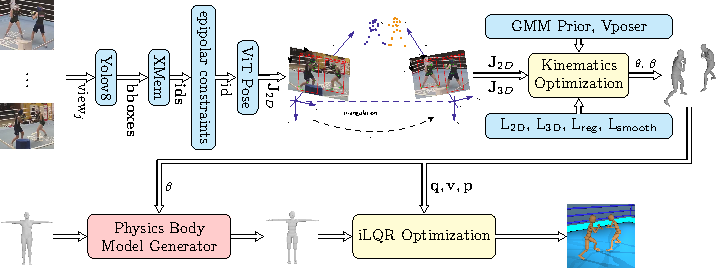
\includegraphics[width=0.9\linewidth]{pipeline.pdf}
%  \centering
%   \caption{The pipeline begins with generating bounding boxes  and robust tracking  for each individual in the scene. These tracking results are used to produce 2D poses. The triangulation process, produces smooth 3D keypoints. The kinematics optimization step incorporates the 2D and 3D keypoints, to create the SMPL parameters ($\mathbf{\theta}$, $\mathbf{\beta}$). The 3D relative joint positions, initial pose state  and velocity state of the humanoid, serve as a reference for a dynamic optimizer to correct any artifacts in the motion.}
% \label{fig:teaser}
% }

\maketitle
%-------------------------------------------------------------------------

\begin{abstract}
   This paper introduces a novel framework for 3D pose estimation in combat sports. Utilizing a sparse multi-camera setup, our approach employs a computer vision-based tracker to extract 2D pose predictions from each camera view, enforcing consistent tracking targets across views with epipolar constraints and long-term video object segmentation. Through a top-down transformer-based approach, we ensure high-quality 2D pose extraction. We estimate the 3D position via weighted triangulation, spline fitting and extended Kalman filtering. By employing kinematic optimization and physics-based trajectory refinement, we achieve state-of-the-art accuracy and robustness under challenging conditions such as occlusion and rapid movements. Experimental validation on diverse datasets, including a custom dataset featuring elite boxers, underscores the effectiveness of our approach. Additionally, we contribute a valuable sparring video dataset to advance research in multi-person tracking for sports.


\begin{CCSXML}
<ccs2012>
<concept>
<concept_id>10010147.10010371.10010352.10010381</concept_id>
<concept_desc>Computing methodologies~Pose Estimation</concept_desc>
<concept_significance>300</concept_significance>
</concept>
<concept>
<concept_id>10010147.10010371.10010352.10010382</concept_id>
<concept_desc>Computing methodologies~Motion synthesis</concept_desc>
<concept_significance>300</concept_significance>
</concept>
</ccs2012>
\end{CCSXML}

\ccsdesc[300]{Computing methodologies~Pose Estimation}
\ccsdesc[300]{Computing methodologies~Motion synthesis}


\printccsdesc   
\end{abstract}  
%-------------------------------------------------------------------------
\section{Introduction}
Combat sports present significant challenges for motion capture due to numerous close-proximity interactions and frequently crowded backgrounds. Optical marker-based tracking, while precise in controlled environments, becomes impractical due to dynamic motions and frequent collisions leading to calibration issues. Inertial measurement unit (IMU) based solutions suffer from global positional drift, affecting inter-athlete distances. Monocular vision-based approaches, though freeing athletes from tracking equipment, often lack precision due to frequent occlusions. However, these occlusions can be mitigated by incorporating data from multiple camera viewpoints, a cornerstone of our tracking pipeline.

We propose a multi-stage, multi-view tracking pipeline shown in Fig~\ref{fig:pipeline} designed to reconstruct high-quality 3D motion of athletes engaged in combat sports such as boxing. Our approach integrates 2D keypoints from multiple camera views through kinematic optimization, followed by physics-based trajectory refinement using model predictive control to eliminate non-physical artifacts. 
The contributions of our work are summarized as follows:
\begin{itemize}
    \item A comprehensive multi-camera multi-person physics based pose estimation framework designed for high-quality 3D pose estimation using as few as three cameras.
    \item A robust triangulation technique employing spline fitting and Kalman filtering to generate consistent and smooth 3D positions.
    \item A high-quality dataset of video footage featuring elite boxers during intense sparring sessions. The dataset encompasses various boxing styles, presenting a valuable new benchmark in 3D pose estimation. We will release a portion of the dataset (20 minutes) and motion data obtained to advance research in competitive sports.
\end{itemize}



\label{sec:results} 

\begin{figure*}[htb]
    \centering
    \begin{minipage}[b]{0.32\textwidth}
        \centering
        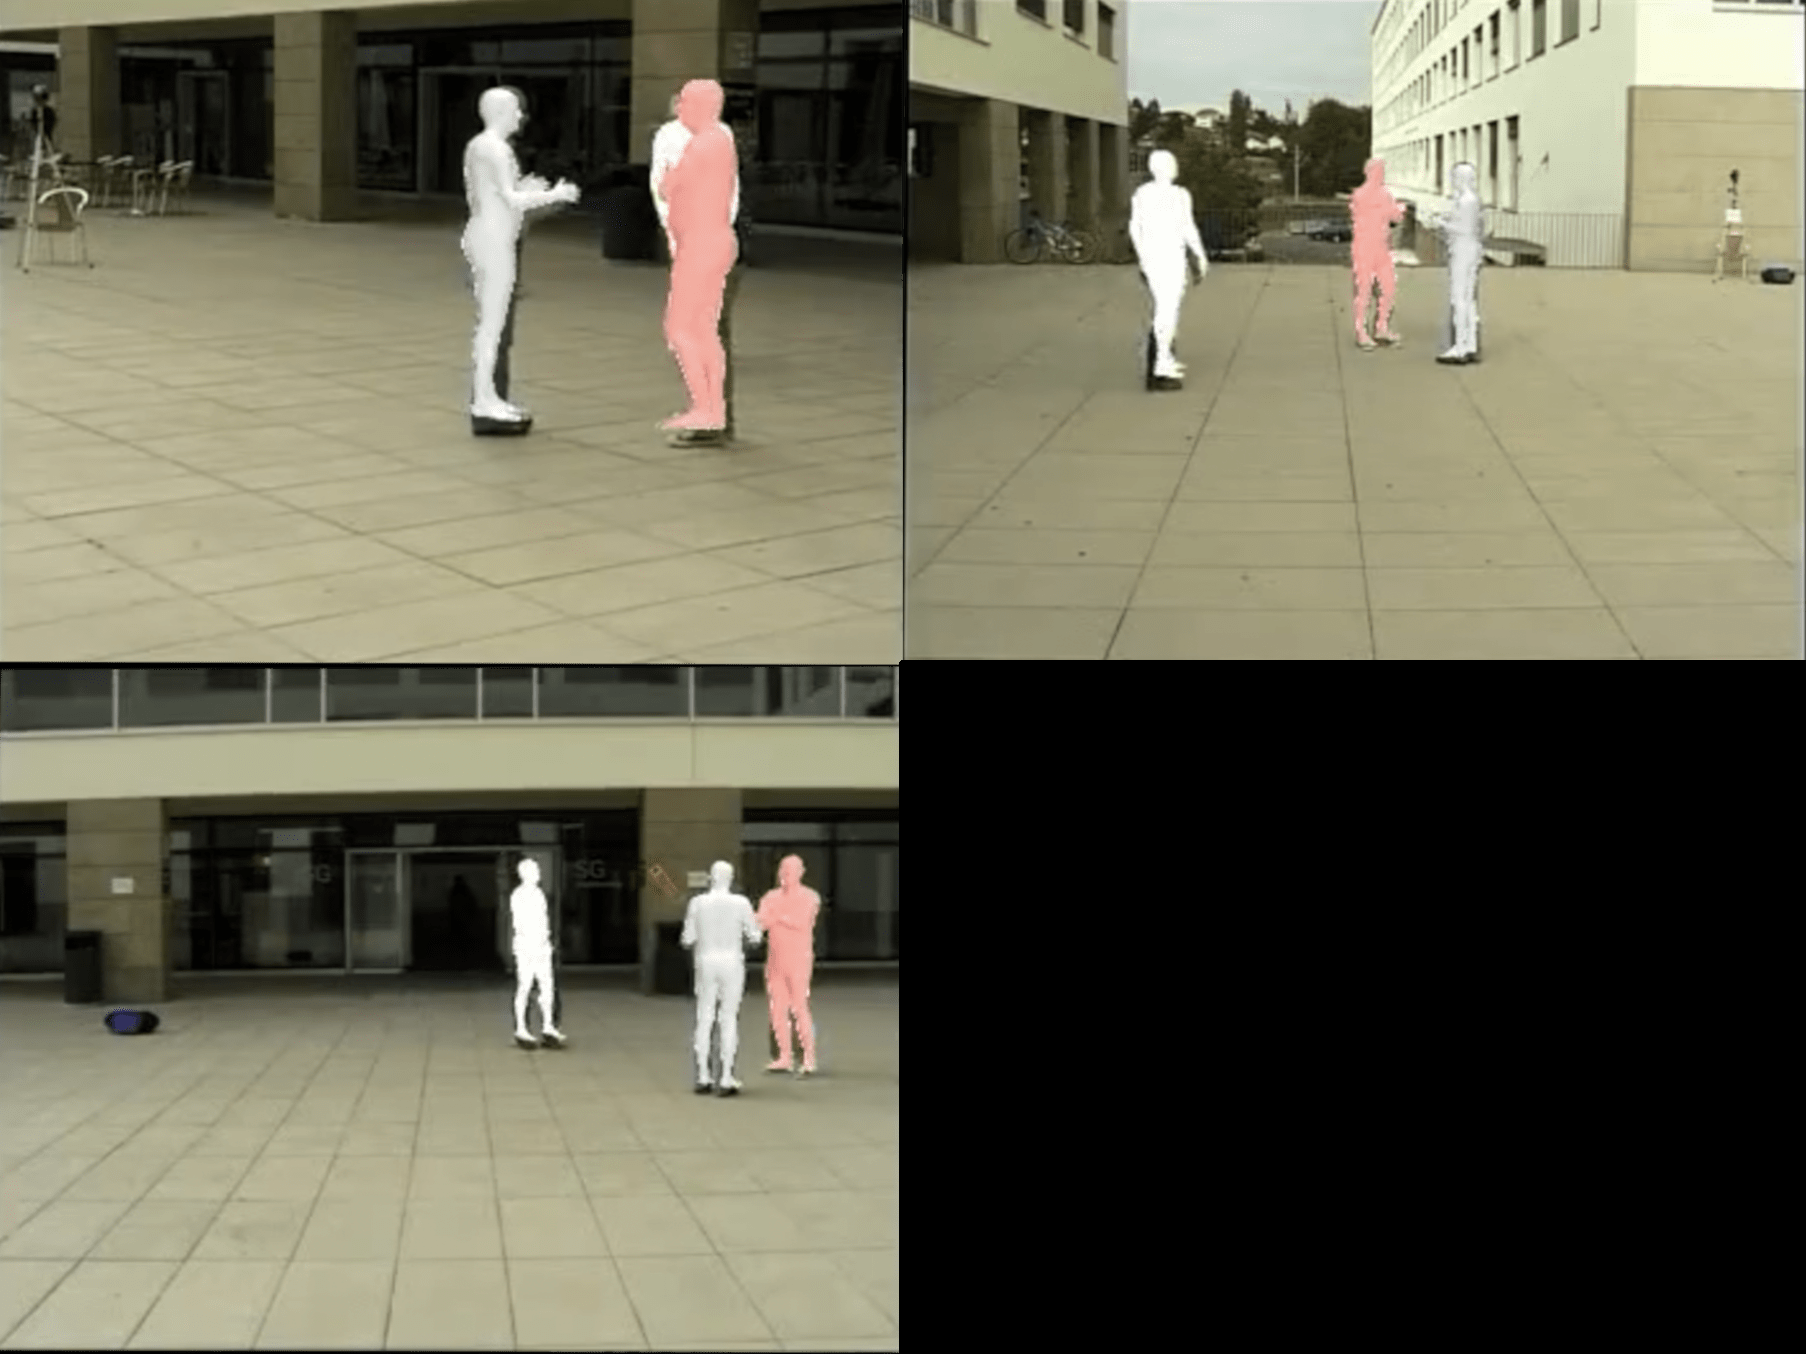
\includegraphics[width=\linewidth]{figures/campus2.png}
    \end{minipage}%
    \hspace{0.01\textwidth}
    \begin{minipage}[b]{0.32\textwidth}
        \centering
        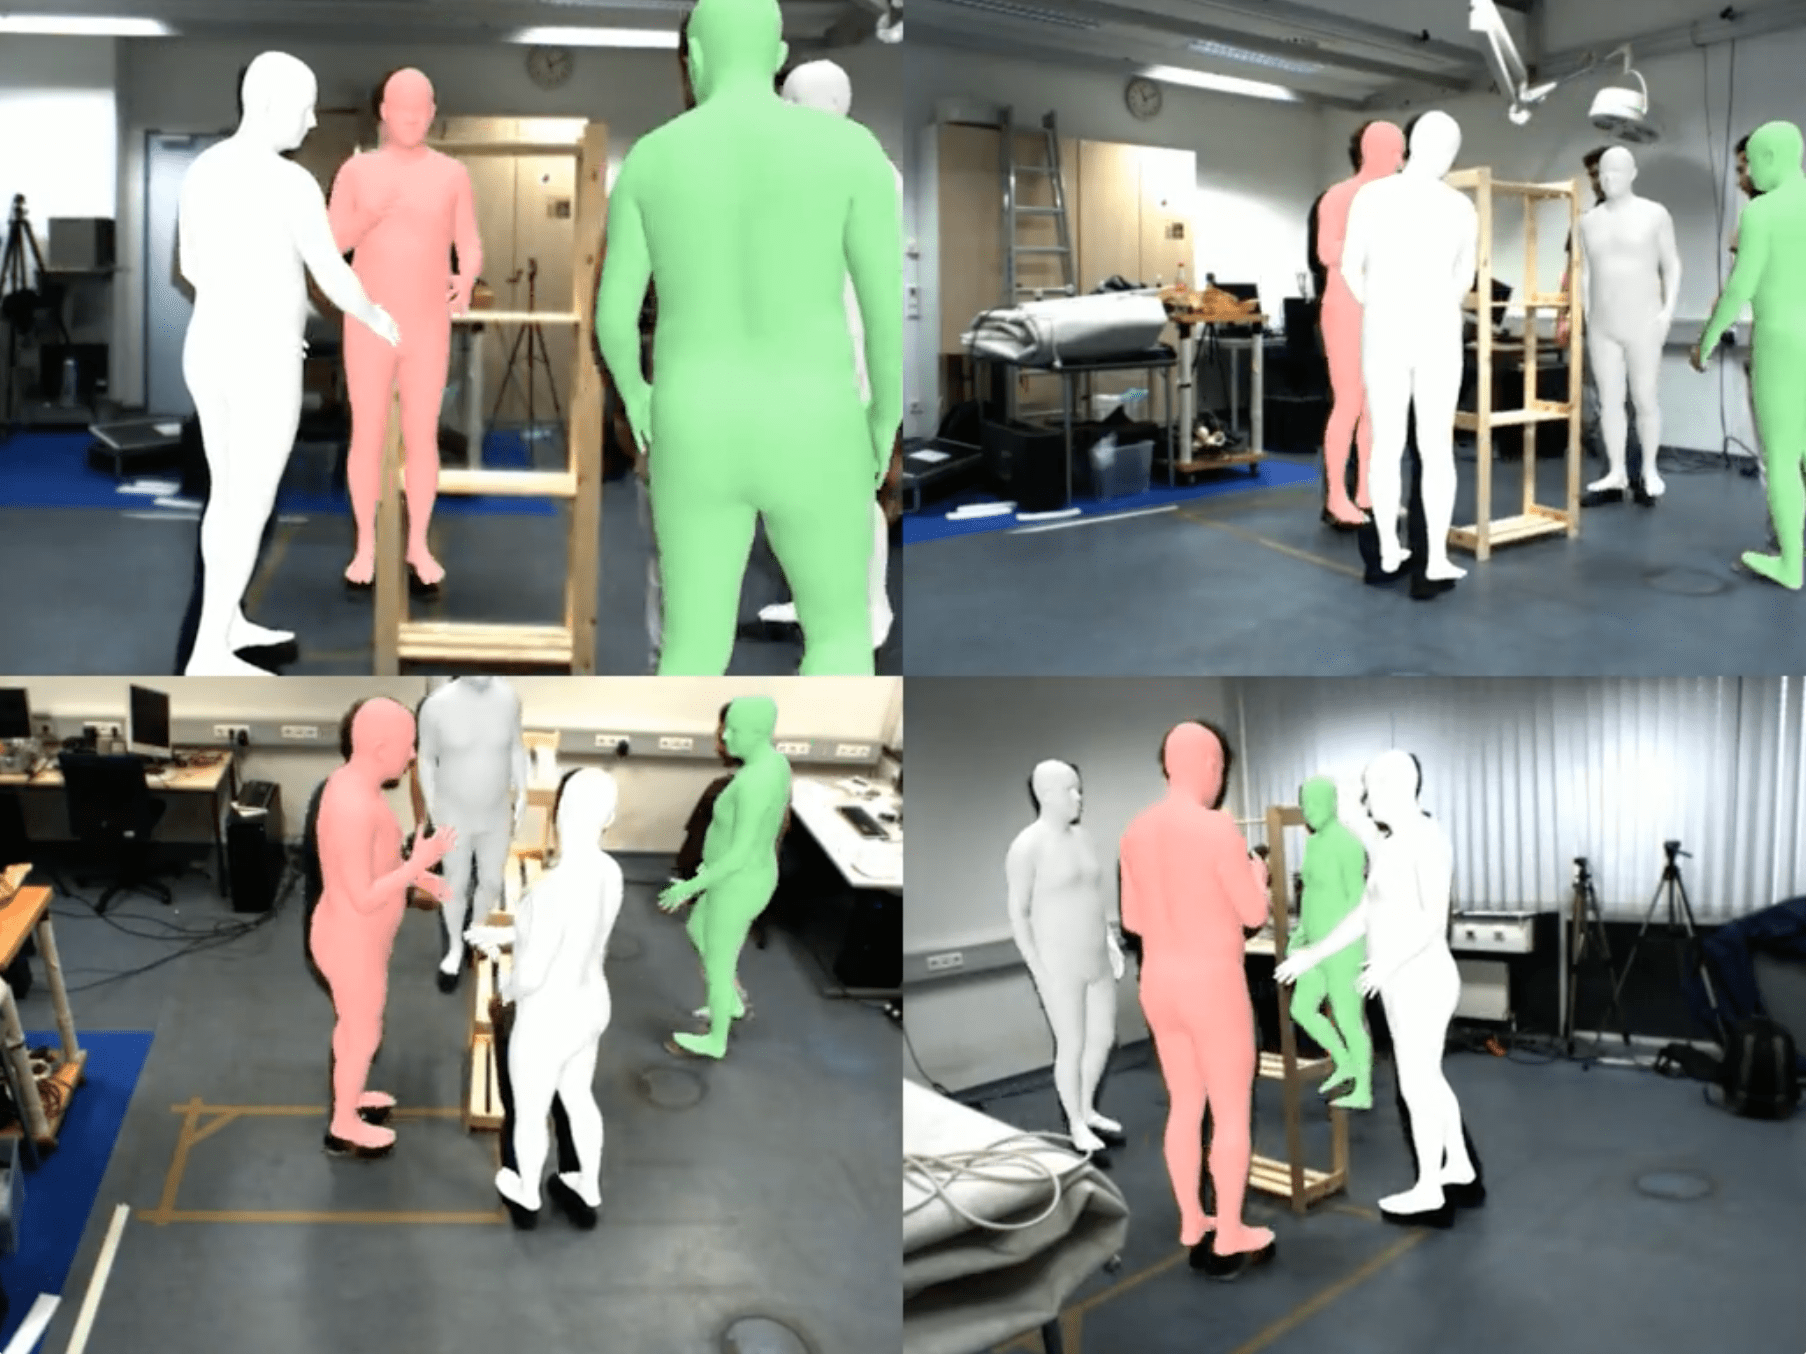
\includegraphics[width=\linewidth]{figures/shelf.png}
    \end{minipage}%
    \hspace{0.01\textwidth}
    \begin{minipage}[b]{0.32\textwidth}
        \centering
        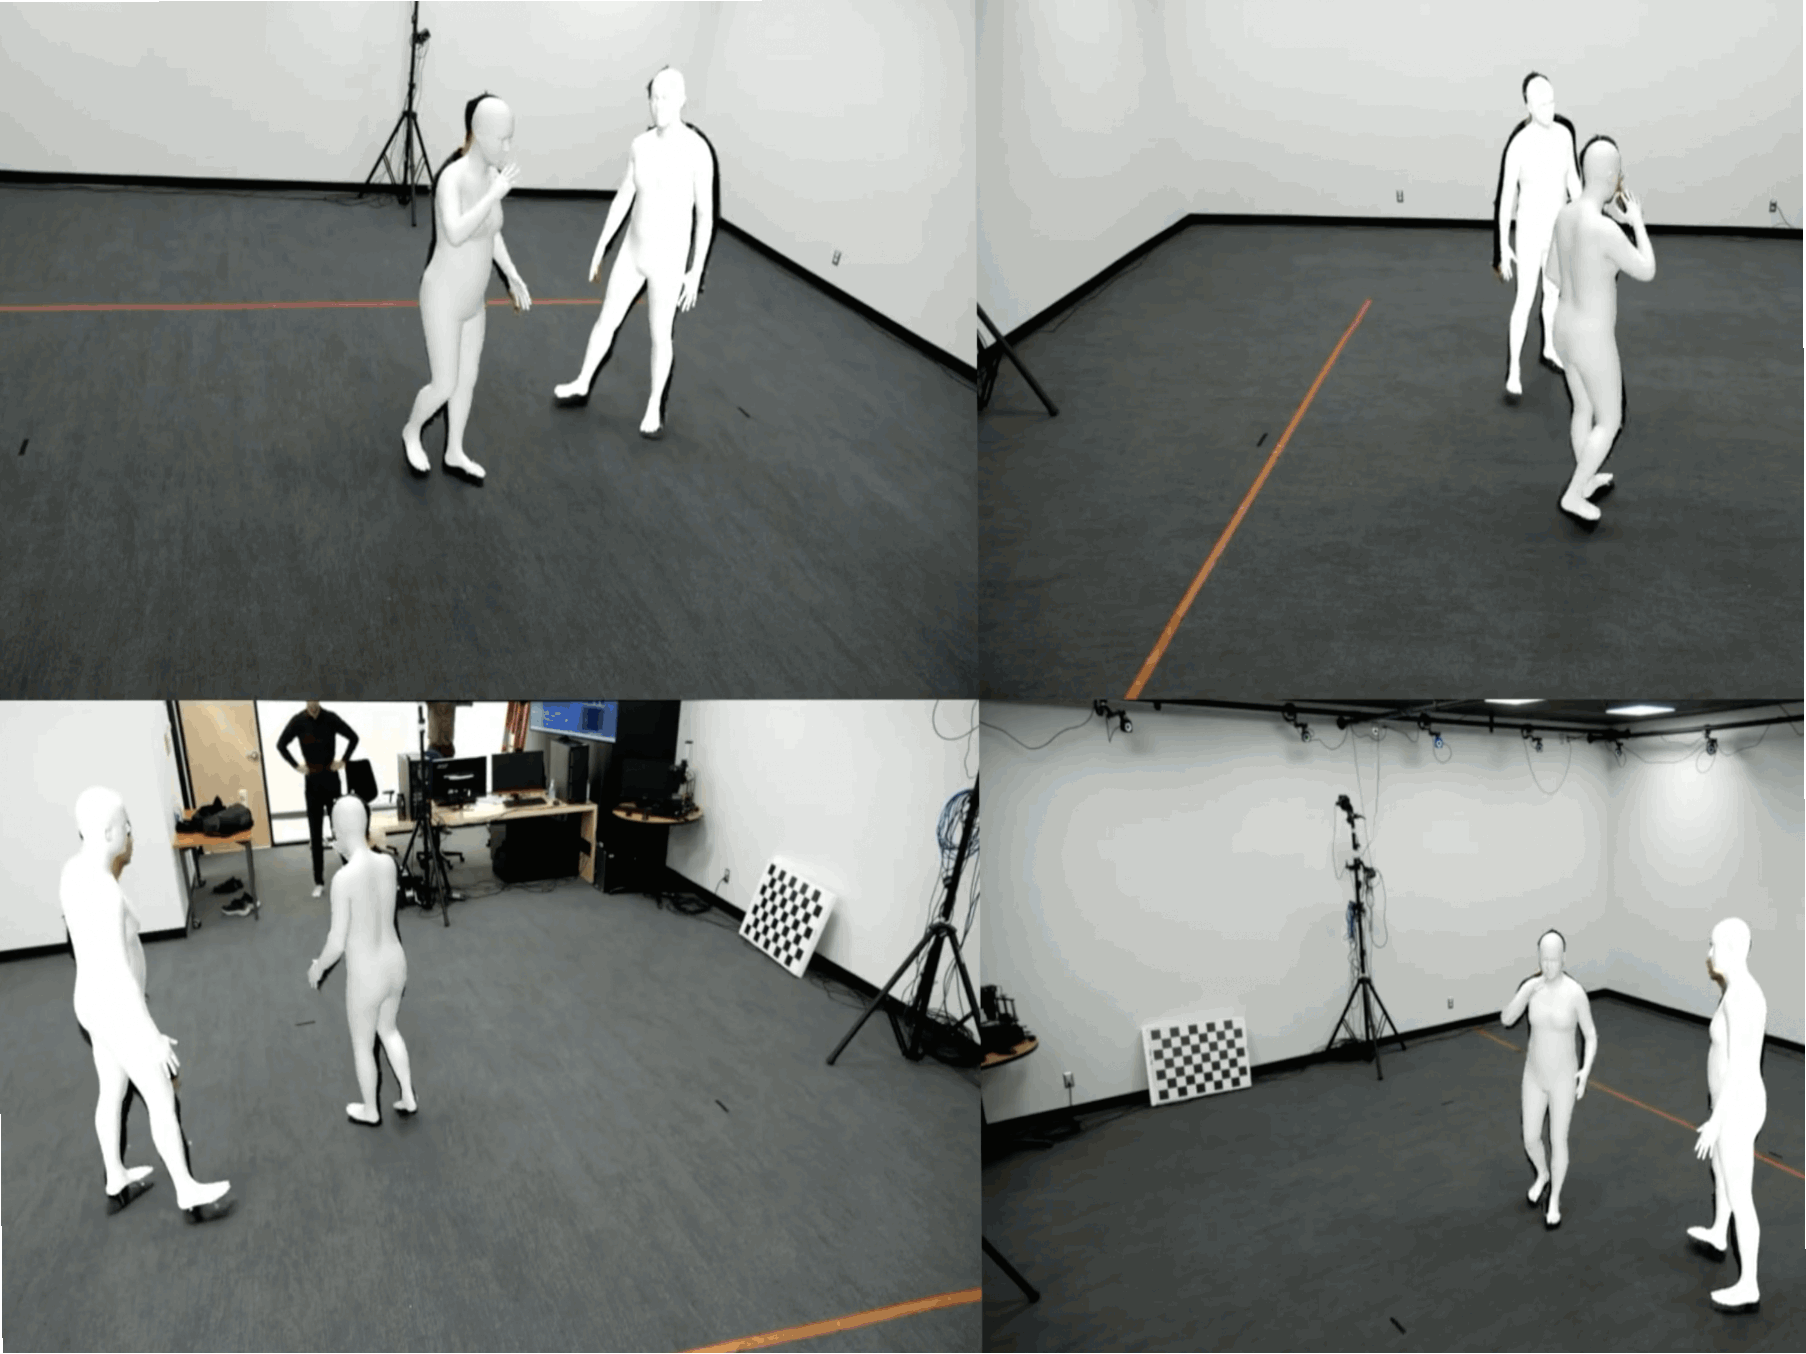
\includegraphics[width=\linewidth]{figures/supp.png}
    \end{minipage}%
    \caption{Poses estimated from the Campus, Shelf and supplementary datasets}
    \label{fig:qualitative}
\end{figure*}
% \begin{table*}[t]
%   \caption{Comparison of PCP[\% $\uparrow$] results on the Campus and Shelf datasets.}
%   \centering
%   \resizebox{\textwidth}{!}{%
%     \begin{tabular}{@{}r|cccc|cccc@{}}
%       \toprule
%       Method & \multicolumn{4}{c|}{Campus} & \multicolumn{4}{c}{Shelf} \\
%       \cmidrule(r){2-5} \cmidrule(l){6-9}
%       & Actor 1 & Actor 2 & Actor 3 & Avg. & Actor 1 & Actor 2 & Actor 3 & Avg.\\
%       \midrule
  
%      ~\cite{wang2021} & 99.3 & 95.1 & 97.8 & 97.4 & 98.2 & 94.1 & 97.4 & 96.6 \\ 
%      ~\cite{yang2023unified} & 98.2 & 94.6 & 98.2 & 97.0 & 99.5 & 96.0 & 97.7 & 97.7 \\       
%       ours (Triangulation) & \textbf{99.6} & 92.2 & 97.6 & 96.5 & \textbf{99.8} & 95.4 & \textbf{98.6} & \textbf{97.9} \\ 
%       ours (Kinematics) & 98.5 & 93.5 & 94.4 & 95.5 & \textbf{99.8} & \textbf{97.6} & \textbf{98.6} & \textbf{98.6} \\
%       ours (Dynamics) & 97.7 & 93.6 & 94.2 & 95.1 & 97.1 & \textbf{97.6} & 97.2 & 97.3 \\
%       \bottomrule
%     \end{tabular}%
%   }
%   \label{tab:benchmark}
% \end{table*}
\section{Pose Estimation}

%-------------------------------------------------------------------------

\textbf{Tracking 2D and 3D Data:} Using epipolar constraints and long-term video object segmentation~\cite{cheng2022xmem} we produce consistent ids for everyone, these ids are used to produce 2D joints positions using~\cite{xu2022vitpose} for tracking targets, we then use linear triangulation and Kalman estimation to produce robust 3D joints positions for each individual even in the presence of noise and outliers.   
\begin{figure*}[!ht]
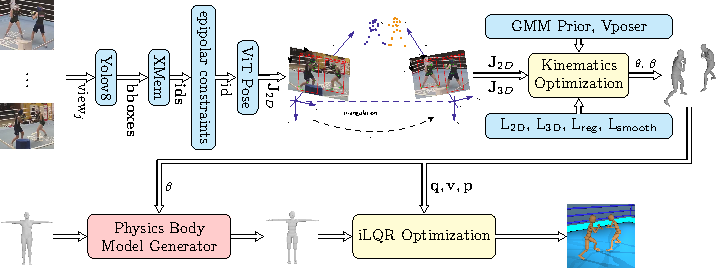
\includegraphics[width=0.75\linewidth]{pipeline.pdf}
 \centering
  \caption{The pipeline begins with generating bounding boxes  and robust tracking  for each individual in the scene. These tracking results are used to produce 2D poses. The triangulation process, produces smooth 3D keypoints. The kinematics optimization step incorporates the 2D and 3D keypoints, to create the SMPL parameters ($\mathbf{\theta}$, $\mathbf{\beta}$). The 3D relative joint positions, initial pose state  and velocity state of the humanoid, serve as a reference for a dynamic optimizer to correct any artifacts in the motion.}
  \label{fig:pipeline}
\end{figure*}

%-------------------------------------------------------------------------

\textbf{Kinematics Optimization:} The kinematics optimization focuses on refining the pose estimation of athletes using 2D and 3D keypoint data. Employing the SMPL model, the optimization aims to minimize the disparity between model joints and observed data while ensuring temporal coherence and natural movement. This is achieved through a comprehensive objective function that includes terms for smoothness, similarity to human motion priors, and alignment with both 2D re-projection evidence and triangulated 3D keypoints.

Initially, the optimization initializes shape parameters ($\beta \in \mathbb{R}^{10}$) of the SMPL model based on 3D keypoints obtained through triangulation. Subsequently, it iteratively adjusts shape and pose parameters ($\theta \in \mathbb{R}^{72}$) to refine the pose estimation.

Key components of the objective function include:

\begin{itemize}
    \item \textbf{2D Re-projection Loss} ($\mathrm{L}_\text{2D}$): Aligns 3D joints with 2D joints across multiple camera views, emphasizing joints with high-confidence detections using a robust error function.
    \item \textbf{3D Alignment Loss} ($\mathrm{L}_\text{3D}$): Computes the Euclidean distance between predicted 3D joint positions and triangulated 3D keypoints, weighted by their confidence scores.
    \item \textbf{Smoothness Loss} ($\mathrm{L}_\text{smooth}$): Promotes consistency in pose transitions over time frames and vertices of the posed mesh.
    \item \textbf{Prior Losses} ($\mathrm{L}_{\text{GMM}}$, $\mathrm{L}_{\text{Vposer}}$): Introduces Gaussian Mixture Model (GMM) and Vposer priors to penalize unnatural poses, guiding the optimization towards more realistic and fluid motion.
\end{itemize}
 This comprehensive approach ensures accurate and lifelike pose estimation suitable for applications in sports biomechanics and animation. Fig~\ref{fig:qualitative} shows the qualitative results of the pipeline on different datasets.

%-------------------------------------------------------------------------

\textbf{Dynamics Optimization:} Output motion of the kinematics optimization contains high-frequency artifacts. To mitigate this, a second stage employs dynamics optimization using a physics-based humanoid model. This model, derived from joint positions and landmarks of an SMPL mesh, creates an articulated rigid-body structure with capsule collision geometry, featuring 56 joint-angle degrees of freedom and a 6 degree of freedom root joint.

The dynamics optimization stage aims to refine motion trajectories by considering joint torques and biomechanical constraints within a physical environment. It computes joint torques using an iterative Linear Quadratic Regulator (iLQR) algorithm~\cite{howell2022}, which optimizes control inputs to smooth and stabilize motion trajectories. This approach accounts for contact forces and body dynamics, enhancing the overall quality and naturalness of the generated motions by iteratively refining control trajectories over short time horizons.



\bibliographystyle{eg-alpha-doi} 
\bibliography{bibliography} 

\end{document}

